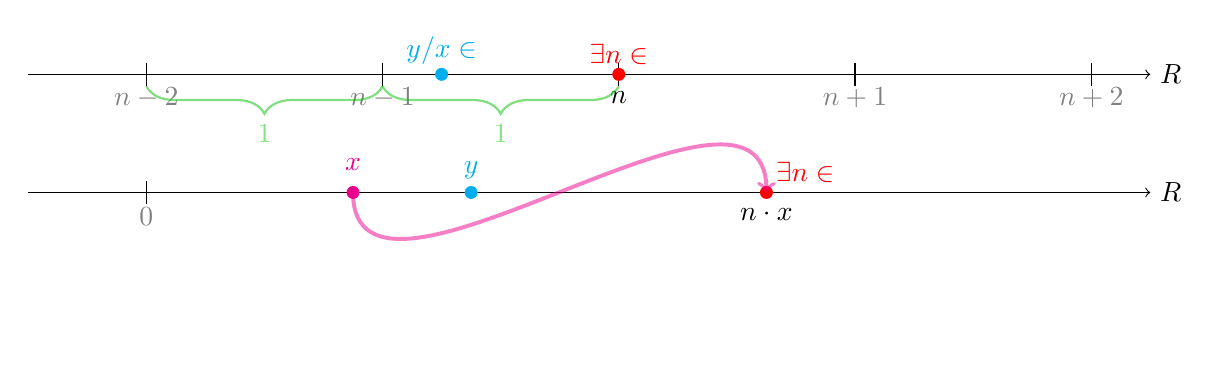
\begin{tikzpicture}[scale=1.5]
	\begin{scope}[yshift=1cm]
	\draw[->] (-1, 0) -- (8.5, 0) node[right] {$\mathbb{R}$};
	
	\foreach \x in {0, 2, ..., 8}
	\draw (\x,0.1) -- (\x,-0.1);
	
	\filldraw[cyan] (2.5, 0) circle (0.05) node[above] {$y/x\in\R$};
	\filldraw[red] (4, 0) circle (0.05) node[above] {$\exists n\in\N$};
	
	\node[gray] at (8,-0.2) {$n+2$};
	\node[gray] at (6,-0.2) {$n+1$};
	\node[] at (4,-0.2) {$n$};
	\node[gray] at (2,-0.2) {$n-1$};
	\node[gray] at (0,-0.2) {$n-2$};
	
	\draw[decorate, decoration={brace, amplitude=10pt}, thick, color=green!75!black, opacity=.5] (4, -0.1) -- (2, -0.1) 
	node[midway, below=10pt, color=green!80!black] {\( 1 \)};	
	\draw[decorate, decoration={brace, amplitude=10pt}, thick, color=green!75!black, opacity=.5] (2, -0.1) -- (0, -0.1) 
	node[midway, below=10pt, color=green!80!black] {\( 1 \)};
	\end{scope}
	% Draw the number line
	\draw[->] (-1, 0) -- (8.5, 0) node[right] {$\mathbb{R}$};
	
	% Mark points on the number line (multiples of x)
	\foreach \n in {0}
	\draw (\n, 0.1) -- (\n, -0.1);
	
	% Mark n * x point
	\filldraw[red] (5.25, 0) circle (0.05) node[above right] {$\exists n\in\N$};
	
%	\node[below, gray] at (8, -0.05) {$(n+1) \cdot x$};
	\node[below] at (5.25, -0.05) {$n \cdot x$};
%	\node[below, gray] at (4, -0.05) {$(n-1) \cdot x$};
%	\node[below, gray] at (2, -0.05) {$(n-2) \cdot x$};
	\node[below, gray] at (0, -0.05) {$0$};
	
	% Mark point y
	\filldraw[cyan] (2.75, 0) circle (0.05) node[above=.05cm] {$y$};
	\filldraw[magenta] (1.75, 0) circle (0.05) node[above=.15cm] {$x$};
	
	\draw[->, line width=.5mm, magenta,out=-90, in=90, opacity=.5] (1.75,0) to (5.25,0);
	
%	\draw[decorate, decoration={brace, amplitude=10pt}, thick, color=green!75!black, opacity=.5] (4, -0.1) -- (2, -0.1) 
%	node[midway, below=10pt, color=green!80!black] {\( x \)};	
%	\draw[decorate, decoration={brace, amplitude=10pt}, thick, color=green!75!black, opacity=.5] (2, -0.1) -- (0, -0.1) 
%	node[midway, below=10pt, color=green!80!black] {\( x \)};
\end{tikzpicture}